\section{Modelo y metodología}

\subsection{Ecuaciones del modelo}
Se considera el siguiente sistema de ecuaciones diferenciales ordinarias no lineales: 

\begin{align}
    \frac{dT}{dt}
    &= R(t)\,T\left(1-\frac{T}{T_{\max}}\right)-\alpha H,
    \\
    \frac{dH}{dt}
    &= \beta T^2-\gamma HP,
    \\
    \frac{dP}{dt}
    &= \delta H^2-\sigma P.
\end{align}

Las variables del modelo son:
\begin{itemize}
    \item $T(t)$: anomalía de temperatura superficial del mar,
    expresada en ${}^{\circ}\mathrm{C}$.
    \item $H(t)$: anomalía de humedad en la atmósfera baja,
    expresada en unidades de humedad ($\mathrm{u.h.}$).
    \item $P(t)$: variable simplificada asociada a la precipitación
    y nubosidad, expresada en unidades de precipitación
    ($\mathrm{u.p.}$).
\end{itemize}
La tasa de crecimiento térmico está modulada por una excitación estacional de período anual:
\begin{equation}
    R(t)=R_{\mathrm{oce}}+A\cos(\omega t-\pi),
    \qquad
    \omega=\frac{2\pi}{12}\;\mathrm{rad/mes}.
\end{equation}

\subsection{Parámetros nominales}

Los valores nominales de los parámetros se presentan en la Cuadro~\ref{tab:parametros}.

\begin{table}[htbp]
    \centering
    \small
    \caption{Parámetros nominales del modelo.}
    \label{tab:parametros}
    \begin{tabular}{@{} l p{0.46\textwidth} l @{}}
        \toprule
        Parámetro & Significado físico & Valor nominal \\
        \midrule
        $T_{\max}$
        & Anomalía máxima térmicamente sostenible
        & $4{,}0\;{}^{\circ}\mathrm{C}$ \\[4pt]

        $R_{\mathrm{oce}}$
        & Tasa intrínseca de calentamiento oceánico
        & $0{,}30\;\mathrm{mes}^{-1}$ \\[4pt]

        $\alpha$
        & Coeficiente de enfriamiento por evaporación
        & $0{,}05\;{}^{\circ}\mathrm{C}\,
           \mathrm{mes}^{-1}\,\mathrm{u.h.}^{-1}$ \\[4pt]

        $\beta$
        & Eficiencia de evaporación
        & $0{,}20\;\mathrm{u.h.}\,
           \mathrm{mes}^{-1}\,({}^{\circ}\mathrm{C})^{-2}$ \\[4pt]

        $\gamma$
        & Tasa de consumo de humedad por precipitación
        & $0{,}10\;\mathrm{mes}^{-1}\,\mathrm{u.p.}^{-1}$ \\[4pt]

        $\delta$
        & Eficiencia de conversión de humedad a lluvia
        & $0{,}40\;\mathrm{u.p.}\,
           \mathrm{mes}^{-1}\,\mathrm{u.h.}^{-2}$ \\[4pt]

        $\sigma$
        & Tasa de descarga o disipación sobre el continente
        & $0{,}70\;\mathrm{mes}^{-1}$ \\[4pt]

        $A$
        & Amplitud de la modulación estacional
        & $0{,}45\;\mathrm{mes}^{-1}$ \\[4pt]

        $\omega$
        & Frecuencia angular para un ciclo anual
        & $\dfrac{2\pi}{12}\;\mathrm{rad/mes}$ \\
        \bottomrule
    \end{tabular}
\end{table}


\subsection{Condiciones iniciales e intervalo de integración}

Se utilizan las siguientes condiciones iniciales:
\begin{equation}
    T(0)=1{,}0\;{}^{\circ}\mathrm{C},
    \qquad
    H(0)=0\;\mathrm{u.h.},
    \qquad
    P(0)=0\;\mathrm{u.p.}
\end{equation}

El intervalo de integración es:
\begin{equation}
    0\leq t\leq 60\;\mathrm{meses}.
\end{equation}

\subsection{Metodología numérica}

Para resolver el sistema se utiliza el método de Euler explícito.
Se define el vector de estado:
\begin{equation}
    \mathbf{y}(t)=
    \begin{bmatrix}
        T(t)\\
        H(t)\\
        P(t)
    \end{bmatrix}.
\end{equation}

La aproximación numérica se obtiene mediante:
\begin{equation}
    \mathbf{y}_{n+1}
    =
    \mathbf{y}_n+h\,\mathbf{f}(t_n,\mathbf{y}_n),
    \qquad
    t_n=nh,
\end{equation}
donde $h$ es el paso temporal, expresado en meses.
En cada iteración se actualizan simultáneamente las tres variables,
utilizando los valores del instante anterior.

\par La implementación se realizó en Python, utilizando NumPy para los cálculos numéricos y Matplotlib para la generación de gráficos.

\newpage

\section{Parte 1: Convergencia, orden y estabilidad del método de Euler}

\subsection{Resolución del sistema mediante el método de Euler explícito}

Para poder resolver el sistema, primero discretizamos:
\begin{itemize}
    \item \textbf{Variable independiente:} $t \to t_n = nh$

    \item \textbf{Variables dependientes:}
    
    \begin{itemize}
        \item $T(t_n) \approx u_n$
        \item $H(t_n) \approx v_n$
        \item $P(t_n) \approx z_n$
    \end{itemize}

    \item \textbf{Ecuaciones diferenciales:} aproximamos cada derivada por una diferencia hacia adelante,
    \fbox{$y'(t_n) \approx \dfrac{y_{n+1}-y_n}{h}$}.
    
    \begin{itemize}
        \item $\frac{u_{n+1} - u_n}{h} = R(t_n) u_n (1 - \frac{u_n}{T_{max}} ) - \alpha v_n$
        \item $\frac{v_{n+1} - v_n}{h} = \beta u_n^2 - \gamma v_n z_n$
        \item $\frac{z_{n+1} - z_n}{h} = \delta v_n^2 - \sigma z_n$
    \end{itemize}
    
    \item \textbf{Condiciones iniciales:}

    \begin{itemize}
        \item $u_0 = 1$
        \item $v_0 = 0$
        \item $z_0 = 0$
    \end{itemize}
    
\end{itemize}

Segundo, para cada ecuación diferencial despejamos en su forma de Euler explícito:

\begin{equation}
    \left\{ 
  \begin{array}{ll} 
    u_{n+1} = u_n + h [R(t_n) u_n (1 - \frac{u_n}{T_{max}} ) - \alpha v_n] \\ 
    v_{n+1} = v_n + h [\beta u_n^2 - \gamma v_n z_n] \\
    z_{n+1} = z_n + h [\delta v_n^2 - \sigma z_n]
  \end{array} 
\right.
\end{equation}

Donde la excitación estacional se calcula como:

\begin{center}

$R(t) = Roce + A cos(w t_n - \pi)$, con $w = \frac{2 \pi}{12} $

\end{center}

y, reemplazando los parámetros nominales, nos quedaria:

\begin{center}

$R(t) = 0.30 + 0.45 cos(\frac{2 \pi}{12} t_n - \pi)$

\end{center}

Y, por último, el intervalo de integracion:

\begin{center}

$0 \le t \le 60$

\end{center}

\subsection{Obtención de una solución “de referencia”}

Elegimos un paso $h_{\mathrm{ref}}$ lo suficientemente pequeño para que
su error sea despreciable frente al de las discretizaciones que
analizaremos posteriormente:

\begin{equation}
    \boxed{h_{\mathrm{ref}}=\frac{12}{2^{18}}\approx
    4{,}577636719\times10^{-5}\;\mathrm{meses}}.
\end{equation}

Al reemplazar $h$ por $h_{\mathrm{ref}}$ en las ecuaciones de Euler explícito, queda
\[
\left\{
\begin{aligned}
    u_{n+1} &= u_n+h_{\mathrm{ref}}\left[R(t_n)u_n\left(1-\frac{u_n}{T_{\max}}\right)-\alpha v_n\right],\\
    v_{n+1} &= v_n+h_{\mathrm{ref}}\left[\beta u_n^2-\gamma v_nz_n\right],\\
    z_{n+1} &= z_n+h_{\mathrm{ref}}\left[\delta v_n^2-\sigma z_n\right].
\end{aligned}
\right.
\]

Para asegurarnos que el error sea, en efecto, despreciable, hacemos una verificación con $h_{ref}$, $2h_{ref}$ y $4h_{ref}$, y vemos que el orden de convergencia observado es 1.000025 (el estadar de un Euler explícito, que es = 1). A su vez, calculamos la diferencia máxima de T al refinar la referencia, lo que nos da $2{,}08784\times10^{-5}\;{}^\circ\mathrm{C}$, que equivale al $0{,}195$ \% del menor error analizado (objetivo: $<$ 1\%, error despreciable).


\subsection{Error máximo para distintos pasos}
Se usaron pasos $h_k=12/2^k$ meses, con $k$ decreciente de $9$ a $0$.
Cada paso es el doble del anterior y divide exactamente el intervalo de
integración. El error máximo absoluto de la temperatura se definió como:
\begin{equation}
    E(h)=\max_{0\leq n\leq N}
    \left|T_h(t_n)-T_{h_{\mathrm{ref}}}(t_n)\right|,
    \qquad t_n=nh,\qquad N=\frac{60\,\mathrm{meses}}{h}.
    \label{eq:parte1-error}
\end{equation}

\begin{table}[H]
    \centering
    \small
    \caption{Error máximo en $T$ y orden observado para pasos sucesivos. El orden de cada fila se calcula respecto del paso inmediatamente anterior, cuando ambos resultados permiten estimarlo.}
    \label{tab:parte1-convergencia}
    \begin{tabular}{@{} r r r l @{}}
        \toprule
        $h$ [meses] & $E(h)$ [$^\circ\mathrm{C}$] & Orden & Estado \\
        \midrule
        $0{,}0234375$ & $0{,}01070049$ & ---       & Finita \\
        $0{,}046875$  & $0{,}02148585$ & $1{,}00571$ & Finita \\
        $0{,}09375$   & $0{,}04323525$ & $1{,}00882$ & Finita \\
        $0{,}1875$    & $0{,}08735086$ & $1{,}01461$ & Finita \\
        $0{,}375$     & $0{,}1772199$  & $1{,}02065$ & Finita \\
        $0{,}75$      & $0{,}3569070$  & $1{,}01001$ & Finita \\
        $1{,}5$       & ---            & ---        & Desbordamiento \\
        $3$           & ---            & ---        & Desbordamiento \\
        $6$           & $3{,}05492\times 10^{25}$ & --- & Espuria y finita \\
        $12$          & $1{,}13879\times 10^{4}$  & --- & Espuria y finita \\
        \bottomrule
    \end{tabular}
\end{table}

\subsection{Orden de convergencia observado}
En el régimen de convergencia se espera que $E(h)\approx C h^p$. Como
los pasos se duplicaron, se estimó el orden mediante
\begin{equation}
    p_{\mathrm{obs}}(2h)=\frac{\log\bigl(E(2h)/E(h)\bigr)}{\log 2}.
    \label{eq:parte1-orden}
\end{equation}

Por ejemplo, al duplicar el menor paso de la
Cuadro~\ref{tab:parte1-convergencia}, el error pasó de $0{,}01070049$ a
$0{,}02148585\;{}^\circ\mathrm{C}$, lo que da $p_{\mathrm{obs}}=1{,}00571$.
Además, el ajuste de $\log E$ frente a $\log h$ con los cuatro pasos más
chicos dio una pendiente de $1{,}00963$. Ambos valores son cercanos a $1$,
que es el orden esperado para Euler explícito. Esto significa que, en este
rango, al reducir $h$ a la mitad el error de $T$ también se reduce
aproximadamente a la mitad.


\begin{figure}[H]
    \centering
    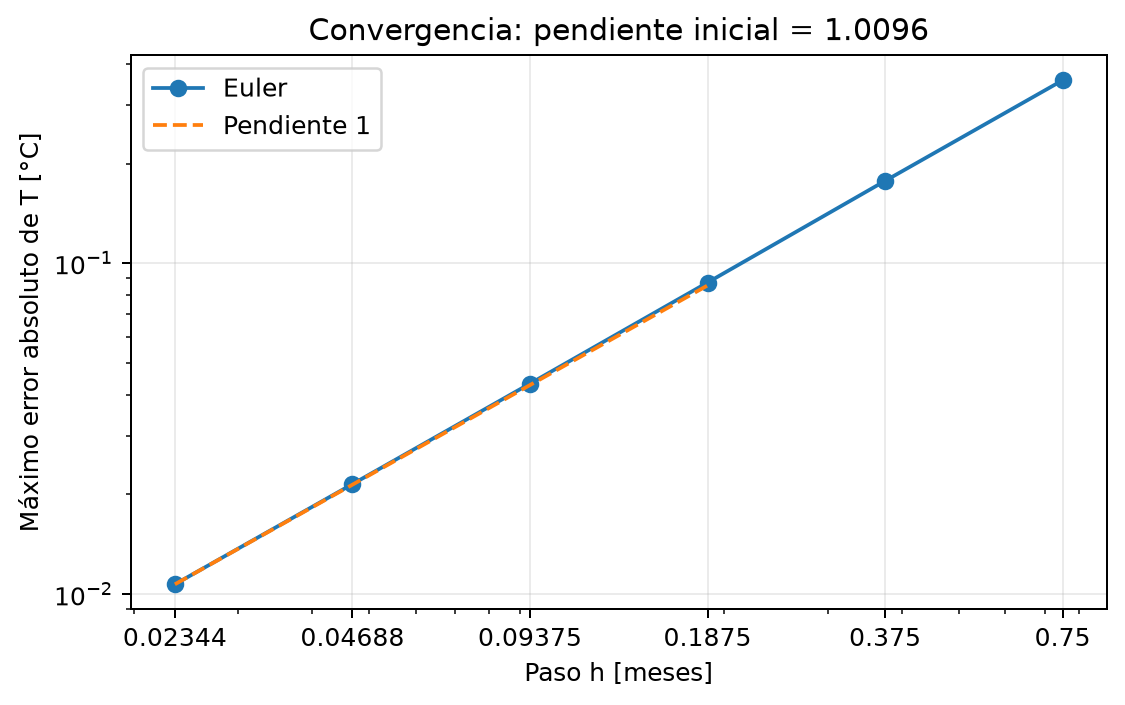
\includegraphics[width=0.85\textwidth]{img/01_convergencia.png}
    \caption{Error máximo absoluto de $T$ en función del paso temporal,
    en escala logarítmica en ambos ejes. La línea discontinua representa
    una dependencia de primer orden.}
    \label{figure:parte1-convergencia}
\end{figure}




\subsection{Estabilidad al aumentar el paso}
Se realizó un barrido auxiliar entre $0{,}25$ y $2$ meses, con un
incremento de $0{,}025$ meses. En este barrido se interpoló linealmente
la referencia en los tiempos de cada simulación cuando las mallas no
coincidían. Se examinó el cociente $E(h)/h$, aproximadamente constante
para errores de primer orden, y se compararon las curvas de precipitación
con la de referencia.


\begin{figure}[htbp]
    \centering
    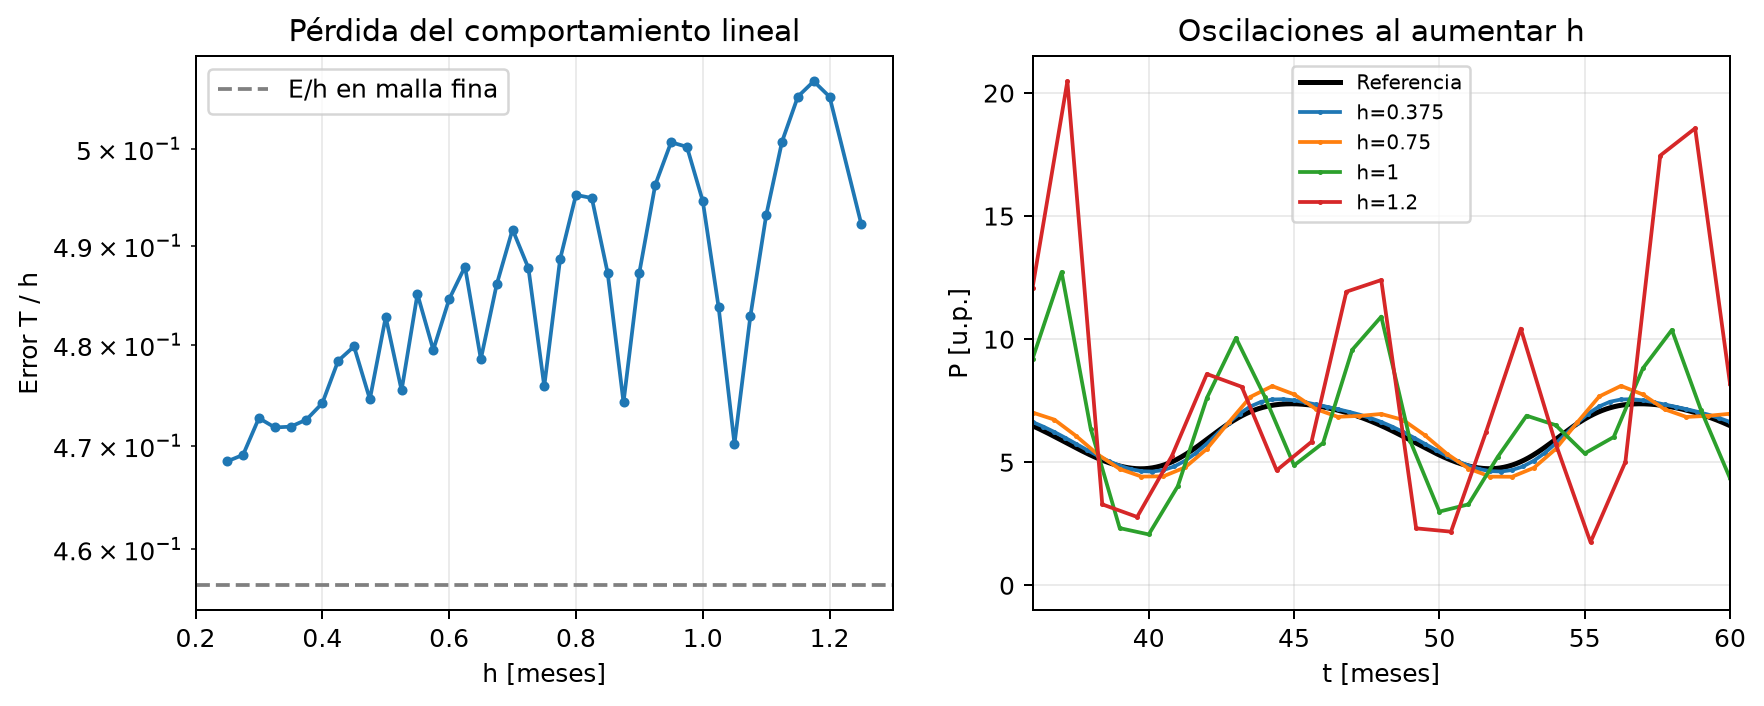
\includegraphics[width=\linewidth]{img/02_estabilidad.png}
    \caption{Cociente $E(h)/h$ para las trayectorias finitas del barrido
    auxiliar (izquierda) y comparación de $P(t)$ entre los meses 36 y 60
    para distintos pasos temporales (derecha).}
    \label{fig:parte1-estabilidad}
\end{figure}

El muestreo anterior no explicaba el crecimiento abrupto del error. Por eso se exploró el intervalo $[1{,}15;\,1{,}30]$ meses con un paso de $0{,}0001$ meses. Entre $h=1{,}1859$ y $h=1{,}1860$ meses, el error máximo de $T$ pasó de aproximadamente $0{,}696$ a
$4{,}42\times 10^{49}\;{}^\circ\mathrm{C}$. En ese segundo caso, la trayectoria ya era explosiva, aunque sus valores todavía se podían representar. El primer desbordamiento apareció en $h=1{,}1865$ meses. 
La Figura~\ref{fig:parte1-detalle} muestra que, en esta zona de
transición, pasos muy cercanos pueden dar comportamientos distintos.
Estos valores dependen de la resolución del barrido y del horizonte de
integración.

\begin{figure}[htbp]
    \centering
    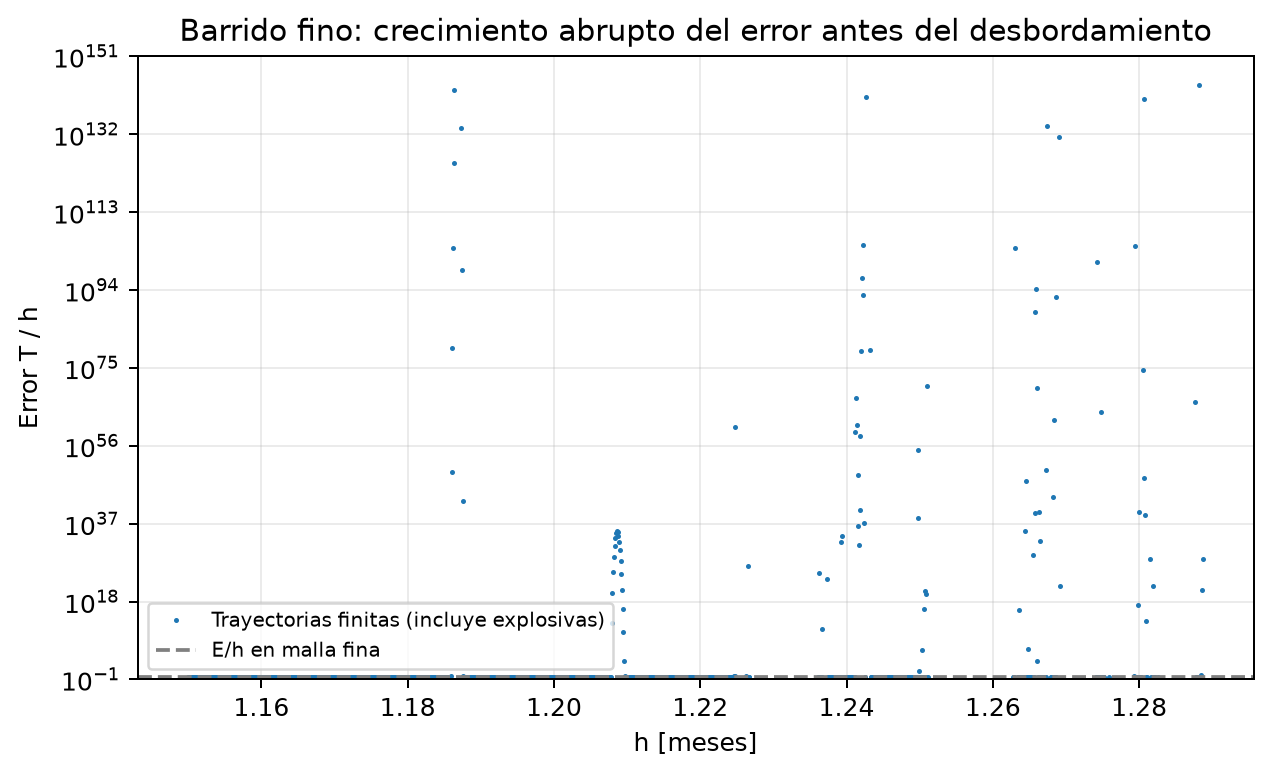
\includegraphics[width=0.90\linewidth]{img/08_estabilidad_detalle.png}
    \caption{Cociente $E(h)/h$ en el barrido fino. Se grafican las trayectorias que llegaron a 60 meses con valores finitos, incluidas las explosivas. Las simulaciones con desbordamiento no aparecen.}
    \label{fig:parte1-detalle}
\end{figure}

Para entender las oscilaciones, se linealizó el sistema alrededor de la trayectoria nominal. En un instante fijo, si $J$ es el jacobiano, una perturbación se propaga aproximadamente con la matriz $I+hJ$. Para un autovalor $\lambda$ de $J$ con parte real negativa, la condición
$|1+h\lambda|\leq 1$ da el límite local
\begin{equation}
    h\leq -\frac{2\operatorname{Re}(\lambda)}{|\lambda|^2}.
\end{equation}

El menor de estos límites, calculado en el último año de la trayectoria nominal, fue de aproximadamente $0{,}8422$ meses, y el autovalor que lo determina es complejo. Esto es coherente con lo observado: con $h=1$ y $h=1{,}2$ meses la precipitación ya oscila de forma artificial (Figura~\ref{fig:parte1-estabilidad}), y el salto abrupto del error aparece poco por encima de ese límite, cerca de $h=1{,}186$ meses. El límite es algo menor que el paso donde se observa el salto porque el cálculo es local: el jacobiano varía a lo largo de la trayectoria y se lo evaluó
``congelado'' en cada instante, de modo que no determina por sí solo la
estabilidad del sistema no lineal.

El error de discretización disminuye al refinar $h$. La inestabilidad
numérica, en cambio, aparece cuando $h$ supera el límite de estabilidad y se
manifiesta como oscilaciones artificiales y crecimiento explosivo, en lugar
de un error que crece de forma gradual con $h$. Una solución finita no es
necesariamente estable ni precisa: con $h=6$ y $h=12$ meses los resultados
fueron finitos, pero incompatibles con la referencia.





\newpage

\section{Parte 2: Severidad estacional, desfase y sensibilidad paramétrica}


\subsection{Selección del paso temporal y análisis general}

Para empezar esta segunda parte, seleccionamos un paso temporal lo suficientemente pequeño para que, de acuerdo con los resultados de la \textbf{Parte 1}, la solución producida sea precisa y estable. A partir de estos mismos resultados, elegimos:

\begin{equation}
    \boxed{h = 0{,}0029296875 \;\mathrm{meses}}.
\end{equation}

En todas las combinaciones exploradas y los barridos individuales, la última comparación h frente a 2h da una diferencia relativa máxima de SP de 0{,}1305\,\% y una diferencia máxima de desfase de 0{,}00878906 meses. Por lo tanto, consideramos el paso seleccionado lo suficientemente bueno para su utilización en los análisis posteriores.

Esta elección es coherente con la Parte~1: $h=12/4096$ es unas $290$ veces menor que el límite local de estabilidad ($0{,}84$ meses), pertenece al rango convergente, donde $E\approx0{,}457\,h$ predice un error máximo de $T$ de unos $1{,}3\times10^{-3}\;{}^\circ\mathrm{C}$, y la diferencia medida entre la simulación nominal con este paso y la referencia fue de $1{,}316\times10^{-3}\;{}^\circ\mathrm{C}$.

Los indicadores se calculan unicamente en el último ciclo anual, definido por el intervalo $48 \le t \le 60$ meses, y se define severidad estacional de las precipitaciones como:

\begin{equation}
    SP = \frac{P_{max} - P_{min}}{P_{med}}
\end{equation}


donde $P_{max}$, $P_{min}$ y $P_{med}$ son los valores máximo, mínimo y promedio de la precipitación durante el ultimo ciclo anual.

Por otra parte, el desfase temperatura-precipitación se calcula como:

\begin{equation}
    \triangle t_{TP} = t_{P,max} - t_{T,max}
\end{equation}

donde $t_{P,max}$ y $t_{T,max}$ corresponde al tiempo en el que se alcanzan la máxima precipitación y temperatura respectivamente.

\subsubsection{Comportamiento del modelo con los parámetros nominales}

En primer lugar, se decidió encontrar los SP y $\triangle t_{TP}$ y graficar T(t), H(t) y P(t) para los 60 meses de la simulación, con resultados:

Con los parámetros nominales, la simulación produce un ciclo anual
prácticamente repetitivo hacia el final del intervalo de integración. El
residuo anual máximo fue $4{,}05\times10^{-4}$, valor inferior al umbral
adoptado de $0{,}01$.

\begin{table}[H]
    \centering
    \small
    \caption{Indicadores del escenario nominal durante el último ciclo anual.}
    \label{tab:parte2-nominal}
    \begin{tabular}{@{} c c c c c c @{}}
        \toprule
        $SP$ & $\Delta t_{TP}$ [meses] & $P_{\max}$ [u.p.] &
        $P_{\min}$ [u.p.] & $P_{\mathrm{med}}$ [u.p.] &
        Residuo anual \\
        \midrule
        $0{,}428658$ & $0{,}826172$ & $7{,}37594$ &
        $4{,}73548$ & $6{,}15985$ & $4{,}05214\times10^{-4}$ \\
        \bottomrule
    \end{tabular}
\end{table}

El máximo de precipitación ocurre aproximadamente $0{,}83$ meses después
del máximo de temperatura. Esto es consistente con la estructura del
modelo, ya que el aumento de temperatura incrementa la humedad mediante
el término $\beta T^2$, y posteriormente la humedad alimenta la variable
de precipitación mediante el término $\delta H^2$.

\begin{figure}[H]
    \centering
    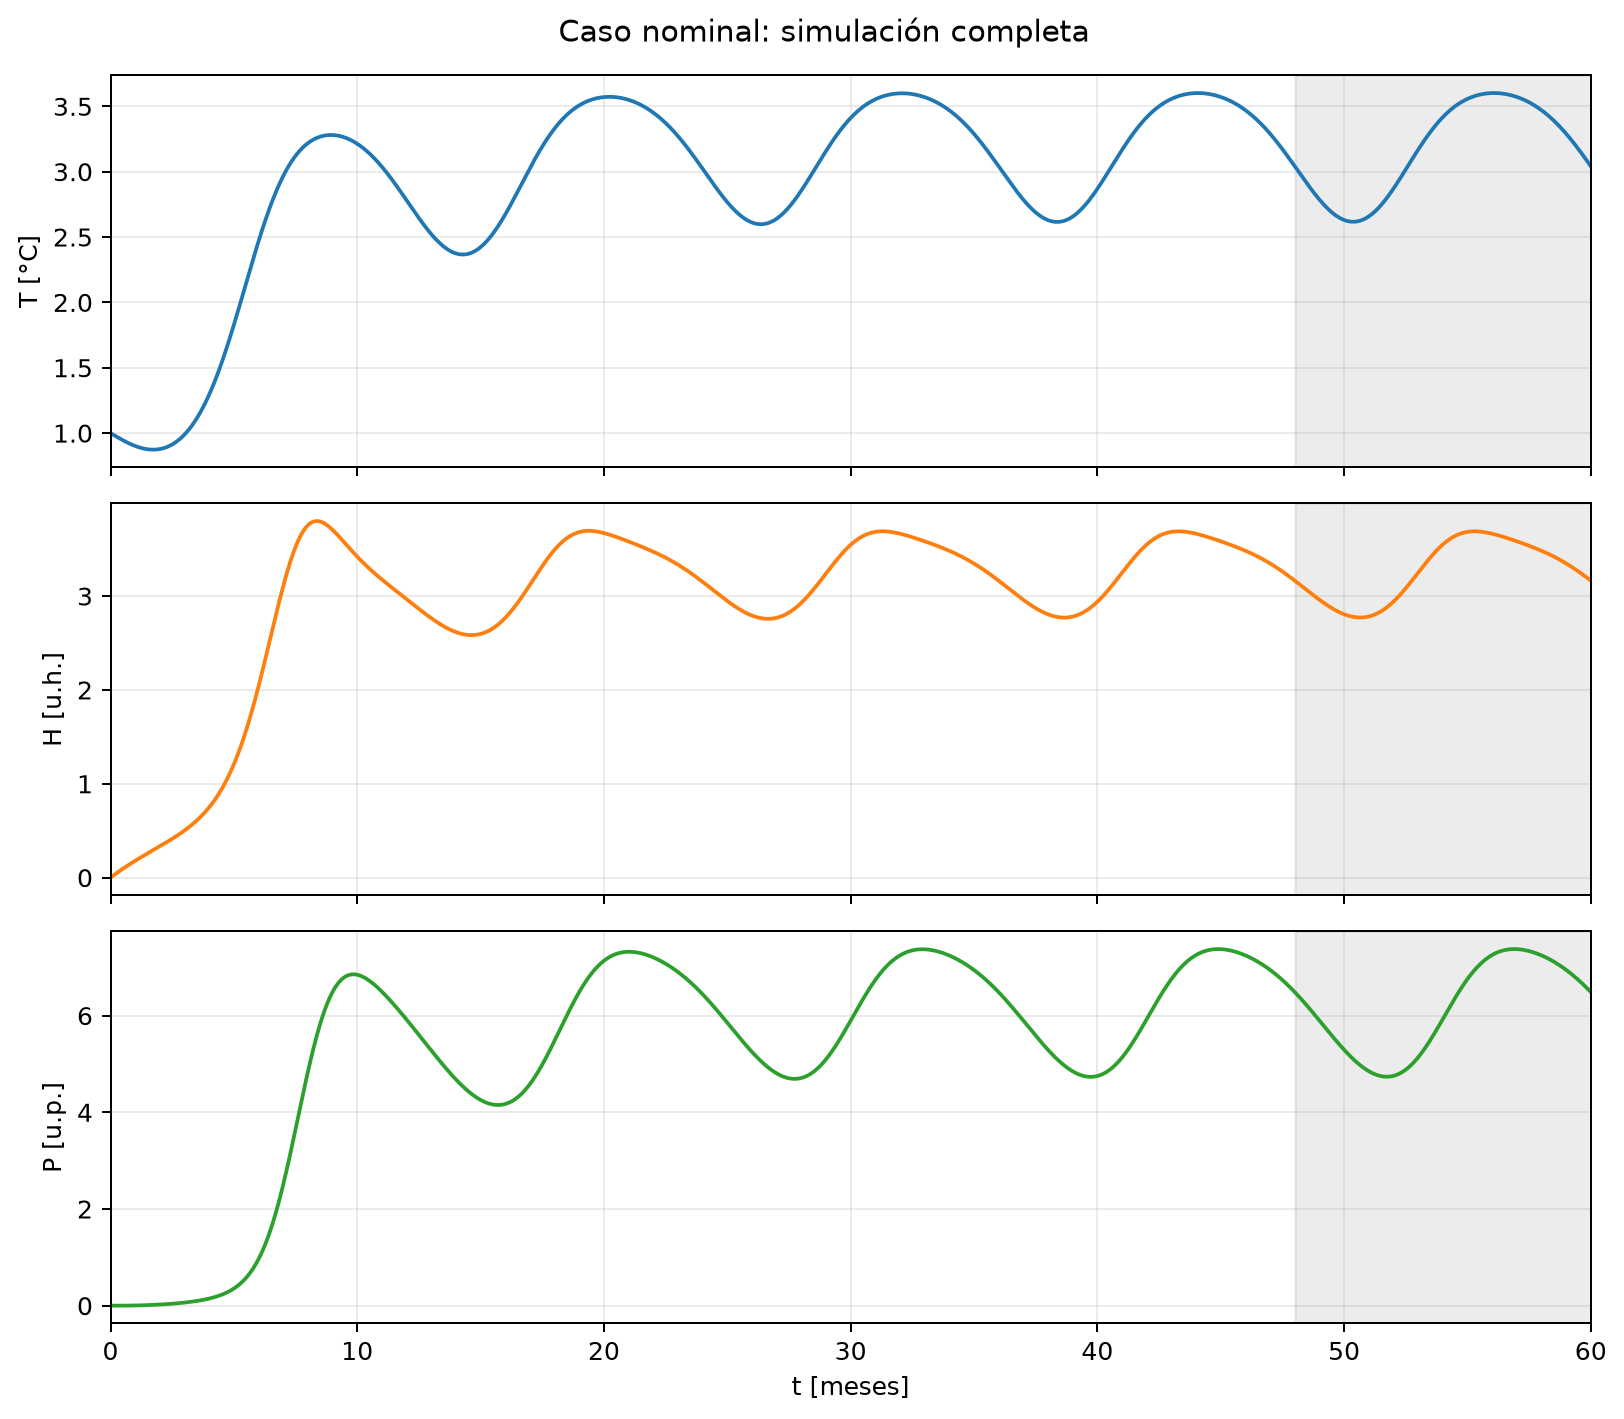
\includegraphics[width=\linewidth]{img/03_nominal_60_meses.png}
    \caption{Evolución temporal de $T(t)$, $H(t)$ y $P(t)$ durante los
    $60$ meses de simulación para los parámetros nominales.}
    \label{fig:parte2-nominal-completo}
\end{figure}


\begin{figure}[H]
    \centering
    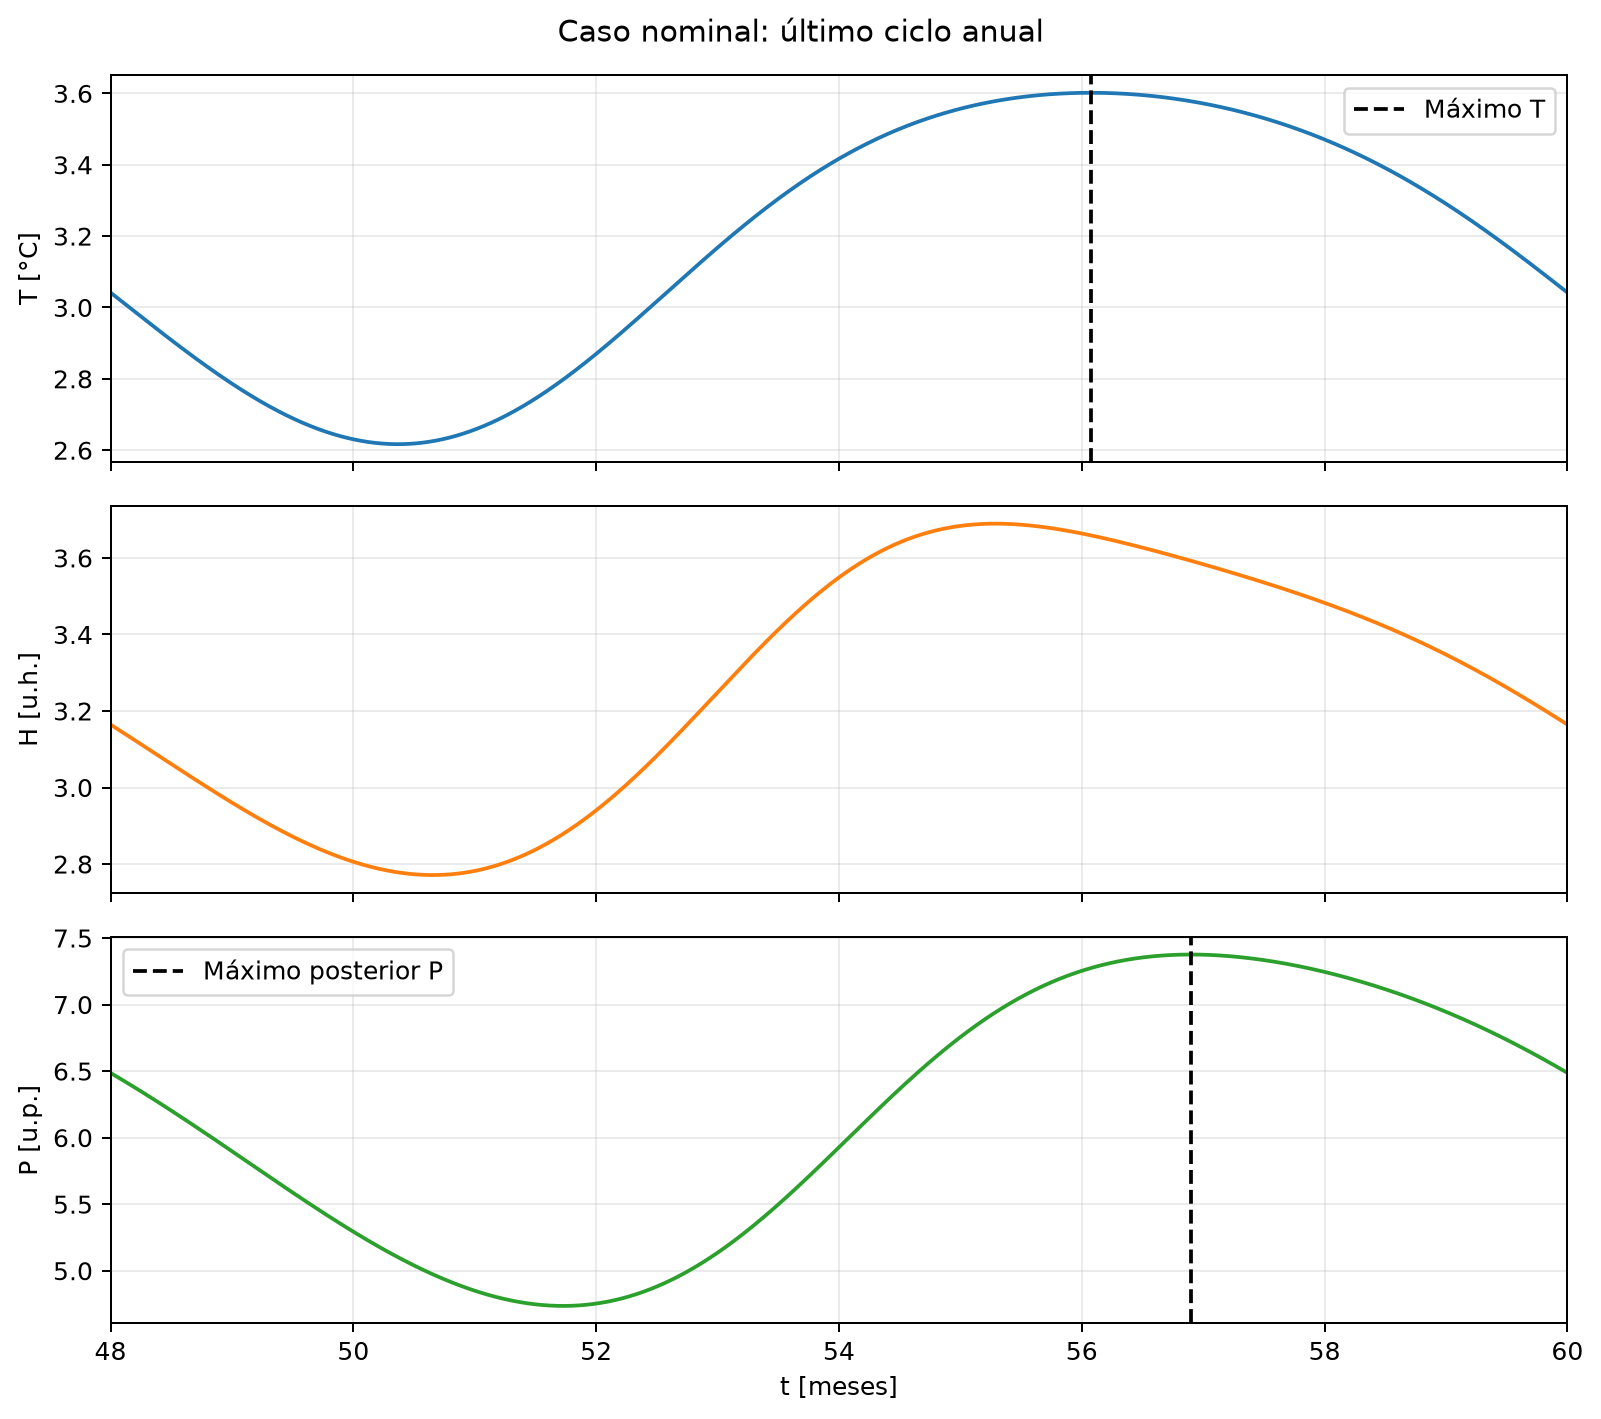
\includegraphics[width=\linewidth]{img/04_nominal_ultimo_ciclo.png}
    \caption{Último ciclo anual del escenario nominal. Se observa el
    desfase entre los máximos de temperatura y precipitación.}
    \label{fig:parte2-nominal-ciclo}
\end{figure}


\subsubsection{Sensibilidad paramétrica individual}

Se estudió la influencia de los parámetros $A$, $\beta$, $\gamma$ y
$\sigma$ sobre la severidad estacional. En cada barrido se modificó un
único parámetro, manteniendo los restantes en sus valores nominales.

\begin{table}[H]
    \centering
    \small
    \caption{Variación de la severidad estacional y del desfase en los
    barridos individuales.}
    \label{tab:parte2-sensibilidad}
    \begin{tabular}{@{} c c c c c @{}}
        \toprule
        Parámetro & Intervalo explorado & $SP$ mínimo & $SP$ máximo &
        Desfase mínimo--máximo [meses] \\
        \midrule
        $A$ & $0{,}25$--$0{,}60$ & $0{,}215492$ & $0{,}626963$ &
        $0{,}735352$--$0{,}955078$ \\
        $\beta$ & $0{,}10$--$0{,}30$ & $0{,}339406$ & $0{,}485561$ &
        $0{,}685547$--$1{,}312500$ \\
        $\gamma$ & $0{,}05$--$0{,}20$ & $0{,}334136$ & $0{,}548950$ &
        $0{,}670898$--$1{,}174805$ \\
        $\sigma$ & $0{,}40$--$1{,}00$ & $0{,}341011$ & $0{,}480803$ &
        $0{,}773438$--$1{,}195312$ \\
        \bottomrule
    \end{tabular}
\end{table}

En los puntos muestreados, SP aumenta con A, $\beta$ y $\sigma$, y disminuye con $\gamma$. El desfase no aumenta al incrementar ninguno de los cuatro parámetros; algunos valores consecutivos coinciden por la resolución temporal de los picos. Estas tendencias se refieren a los intervalos indicados y al resto de parámetros nominales.

\begin{itemize}
        \item A: aumenta el contraste estacional de R(t), sin cambiar su media anual. En los experimentos aumenta SP y disminuye el desfase: la excitación térmica más intensa se propaga a H y P a través de sus fuentes cuadráticas.
        \item $\beta$: aumenta la fuente de humedad $\beta T^2$. En este rango aumenta SP y reduce el desfase, aunque también refuerza el enfriamiento indirecto de T a través de H. El resultado surge del sistema acoplado, no solo del signo positivo de beta.
        \item $\gamma$: aumenta el consumo de humedad $\gamma H P$. Reduce la humedad disponible para la fuente $\delta H^2$. Se observa una menor severidad relativa y un desfase menor; el consumo atenúa el ciclo y acelera el ajuste de humedad cuando P es positiva.
        \item $\sigma$: aumenta la descarga de P y reduce su escala de disipación 1/sigma. En este rango disminuye el desfase y aumenta SP: una disipación más rápida reduce el almacenamiento y permite mayor contraste relativo entre máximo y mínimo. Esto no implica que aumente la precipitación absoluta.
\end{itemize}

\begin{figure}[H]
    \centering
    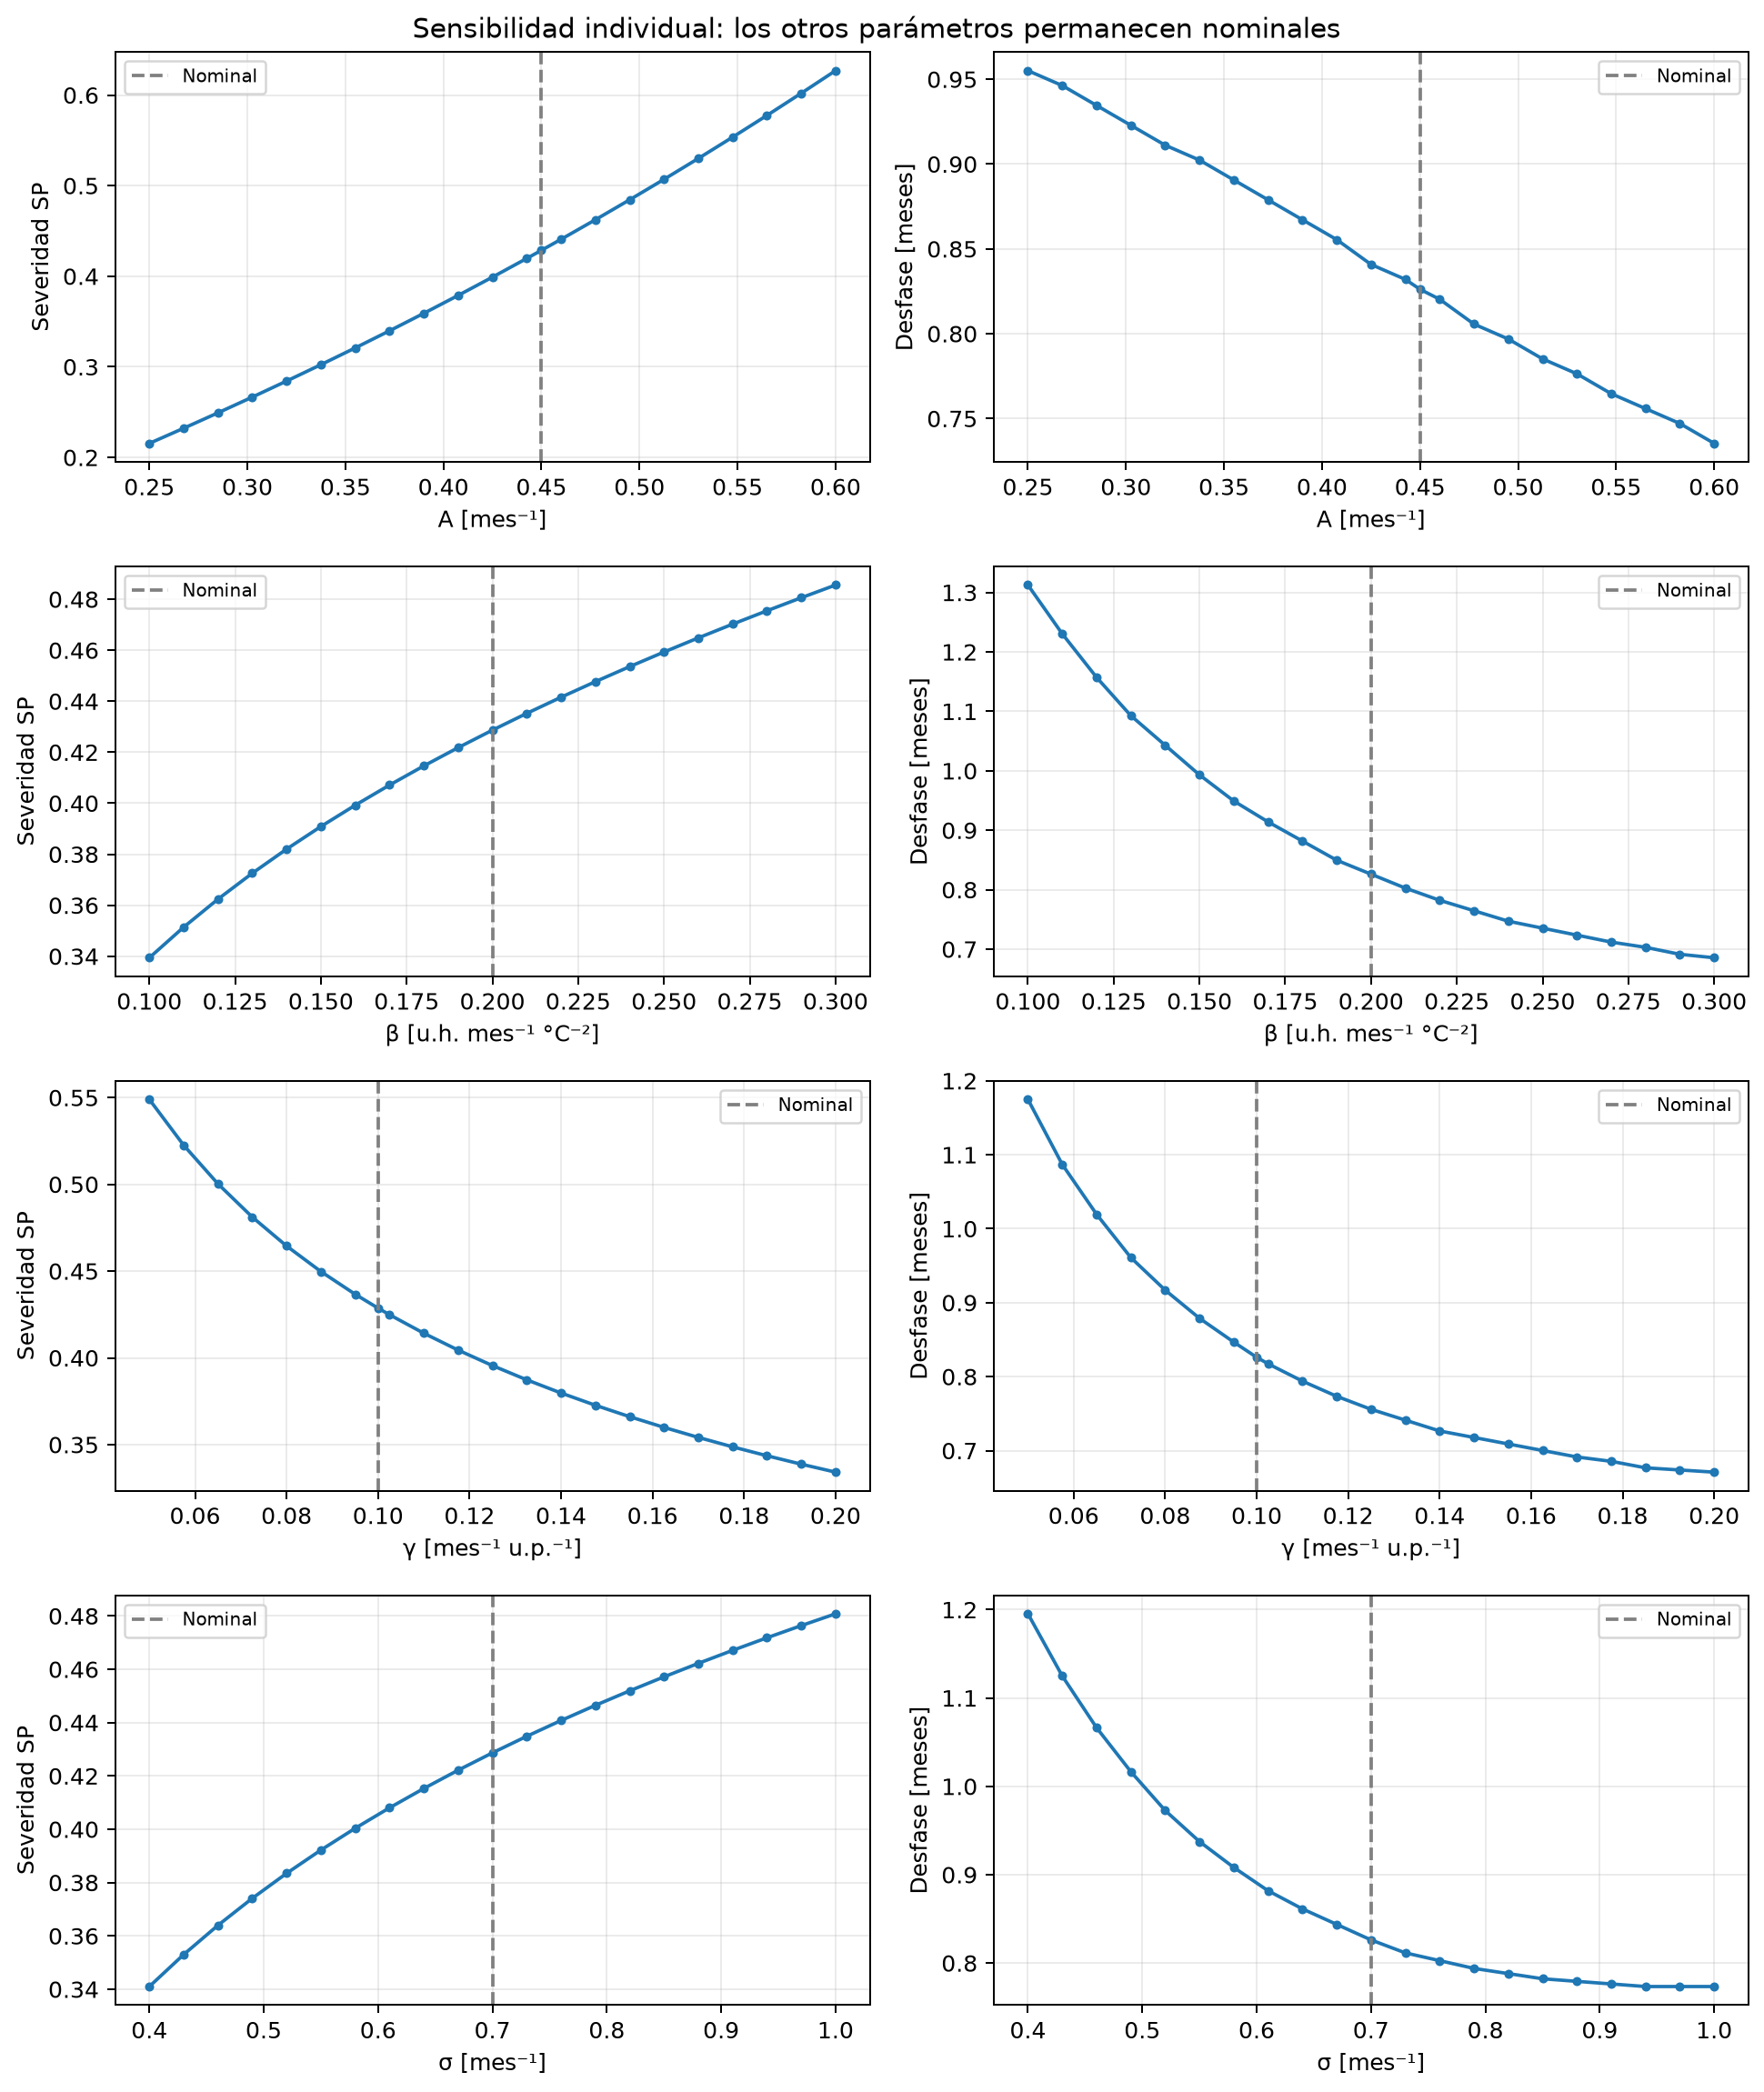
\includegraphics[width=\linewidth]{img/05_sensibilidad.png}
    \caption{Sensibilidad de la severidad estacional y del desfase ante
    variaciones individuales de $A$, $\beta$, $\gamma$ y $\sigma$.}
    \label{fig:parte2-sensibilidad}
\end{figure}


\subsubsection{Búsqueda conjunta y comparación con el escenario nominal}

Luego de los barridos individuales, se modificaron simultáneamente los parámetros $A$, $\beta$, $\gamma$ y $\sigma$ con el objetivo de maximizar la severidad estacional, manteniendo una solución acotada y aproximadamente periódica durante el último ciclo anual.

Se evaluaron 7170 combinaciones distintas entre la grilla inicial de $5^4=625$ puntos, una grilla global de $9^4=6561$ puntos y el refinamiento local de $5^4=625$ puntos eliminando los repetidos. Todas cumplieron el criterio operativo de admisibilidad. El mayor residuo
anual registrado fue $0{,}00110776$ menor que el umbral adoptado de
$0{,}01$.

El residuo compara cada variable del penúltimo y último ciclo a igual fase y normaliza por su máxima magnitud en el último ciclo. La comparación indica repetición anual aproximada al final de los 60 meses; no demuestra periodicidad exacta ni acotación para todo tiempo futuro.

La mejor combinación encontrada fue
\[
    \boxed{
    A=0{,}60,\qquad
    \beta=0{,}30,\qquad
    \gamma=0{,}05,\qquad
    \sigma=1{,}00.}
\]

\begin{table}[H]
    \centering
    \small
    \caption{Comparación de indicadores para distintos escenarios.}
    \label{tab:parte2-comparacion}
    \begin{tabular}{@{} l c c c c c c c c c @{}}
        \toprule
        Escenario & $A$ & $\beta$ & $\gamma$ & $\sigma$ &
        $SP$ & $\Delta t_{TP}$ [meses] & $P_{\max}$ [u.p.] &
        $P_{\min}$ [u.p.] & $P_{\mathrm{med}}$ [u.p.] \\
        \midrule
        Nominal
        & $0{,}45$ & $0{,}20$ & $0{,}10$ & $0{,}70$
        & $0{,}428658$ & $0{,}826172$ & $7{,}376$ & $4{,}736$ & $6{,}160$ \\
        Máxima severidad
        & $0{,}60$ & $0{,}30$ & $0{,}05$ & $1{,}00$
        & $0{,}991270$ & $0{,}893555$ & $12{,}653$ & $4{,}329$ & $8{,}397$ \\
        Todos máximos
        & $0{,}60$ & $0{,}30$ & $0{,}20$ & $1{,}00$
        & $0{,}626015$ & $0{,}439453$ & $5{,}450$ & $2{,}773$ & $4{,}275$ \\
        \bottomrule
    \end{tabular}
\end{table}

El escenario de máxima severidad tiene un valor de $SP$ aproximadamente
$2{,}31$ veces mayor que el escenario nominal. Sin embargo, este resultado
no se obtiene asignando el valor máximo a todos los parámetros.

La mejor combinación usa el valor mínimo de $\gamma$, ya que este parámetro
representa el consumo de humedad por precipitación. Al disminuir $\gamma$,
queda más humedad disponible para generar precipitación y aumenta la
severidad estacional.

De hecho, cuando todos los parámetros toman sus valores máximos se obtiene
$SP=0{,}626015$, un valor menor que el máximo encontrado. Esto muestra que
los parámetros actúan de forma acoplada y que aumentar cada uno por separado
no necesariamente aumenta la severidad estacional.

\begin{figure}[H]
    \centering
    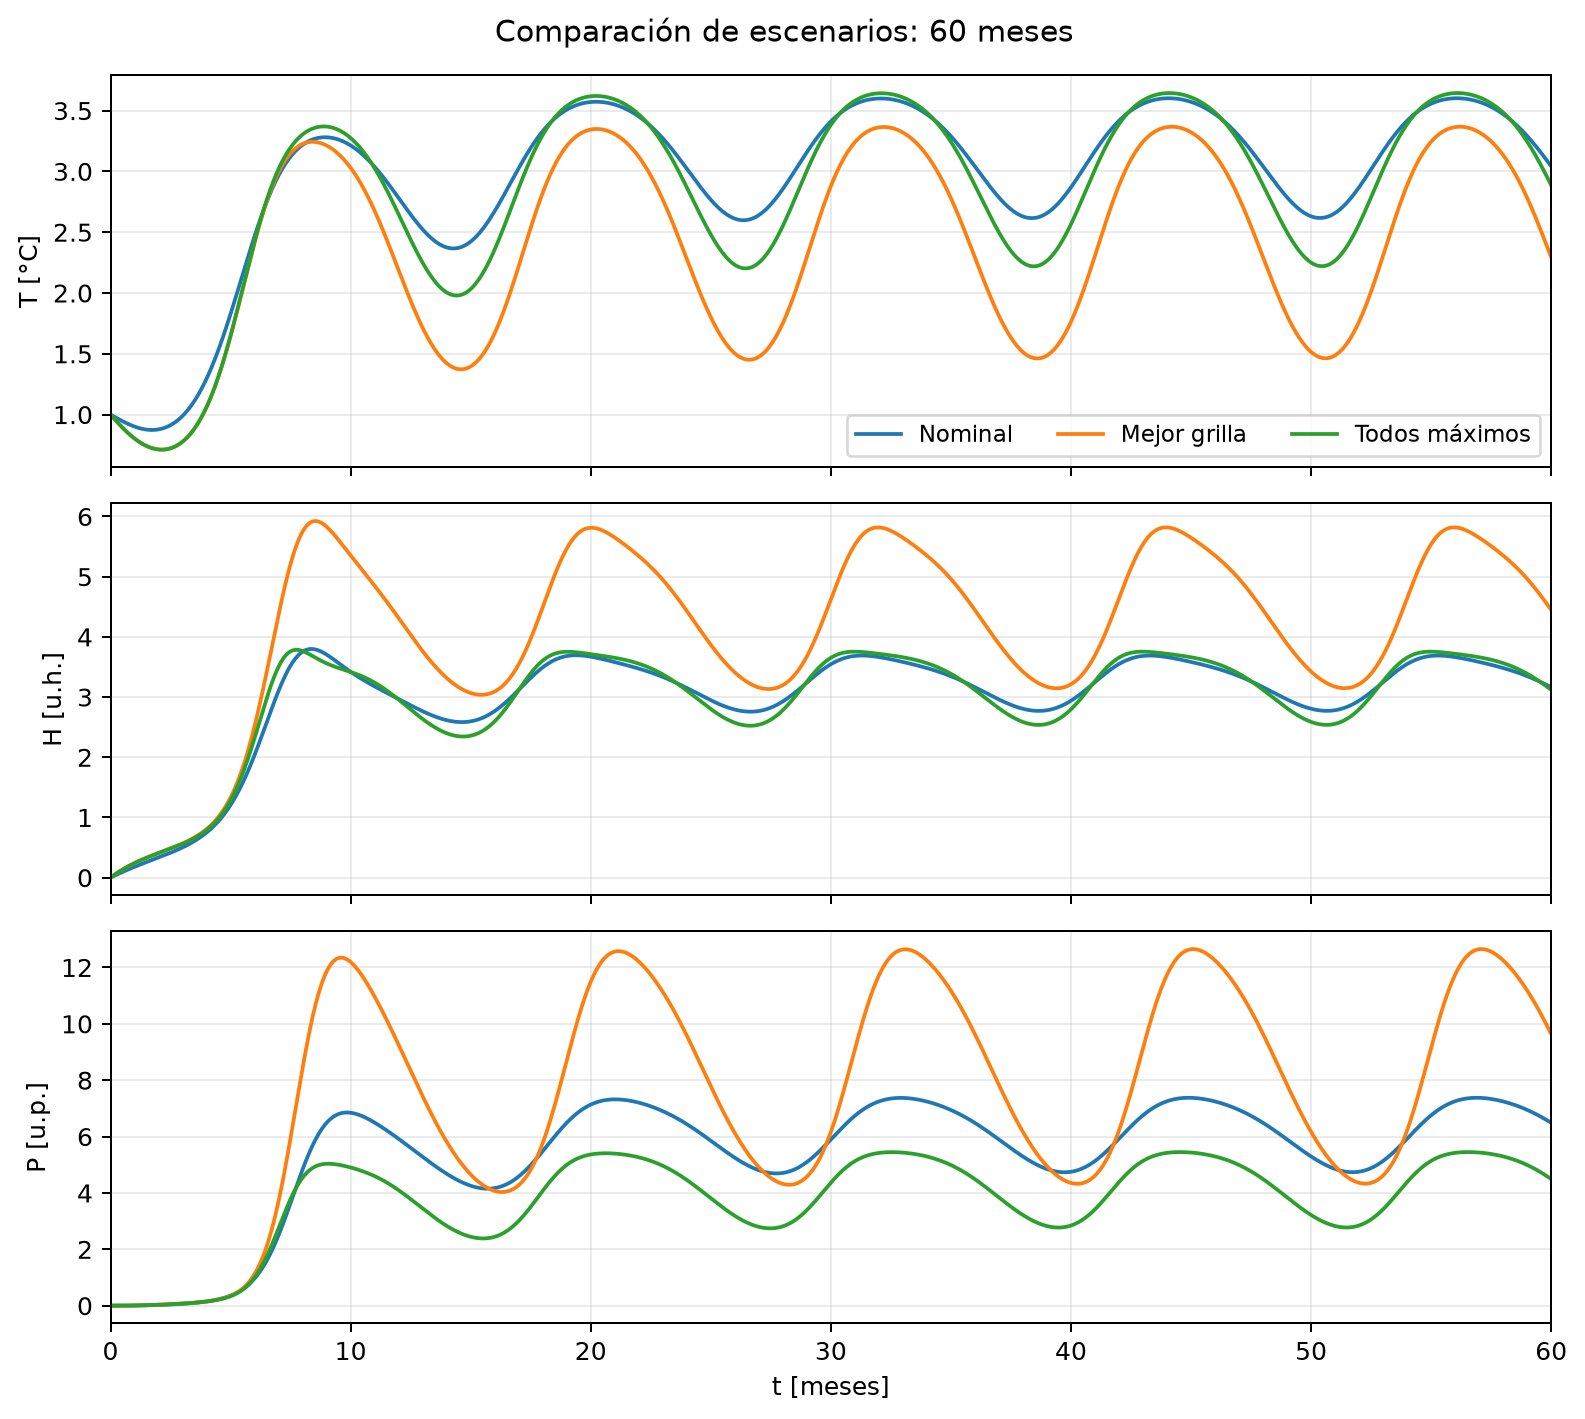
\includegraphics[width=\linewidth]{img/06_comparacion_60_meses.png}
    \caption{Comparación temporal entre el escenario nominal y el
    escenario de máxima severidad durante los $60$ meses simulados.}
    \label{fig:parte2-comparacion-completa}
\end{figure}

\begin{figure}[H]
    \centering
    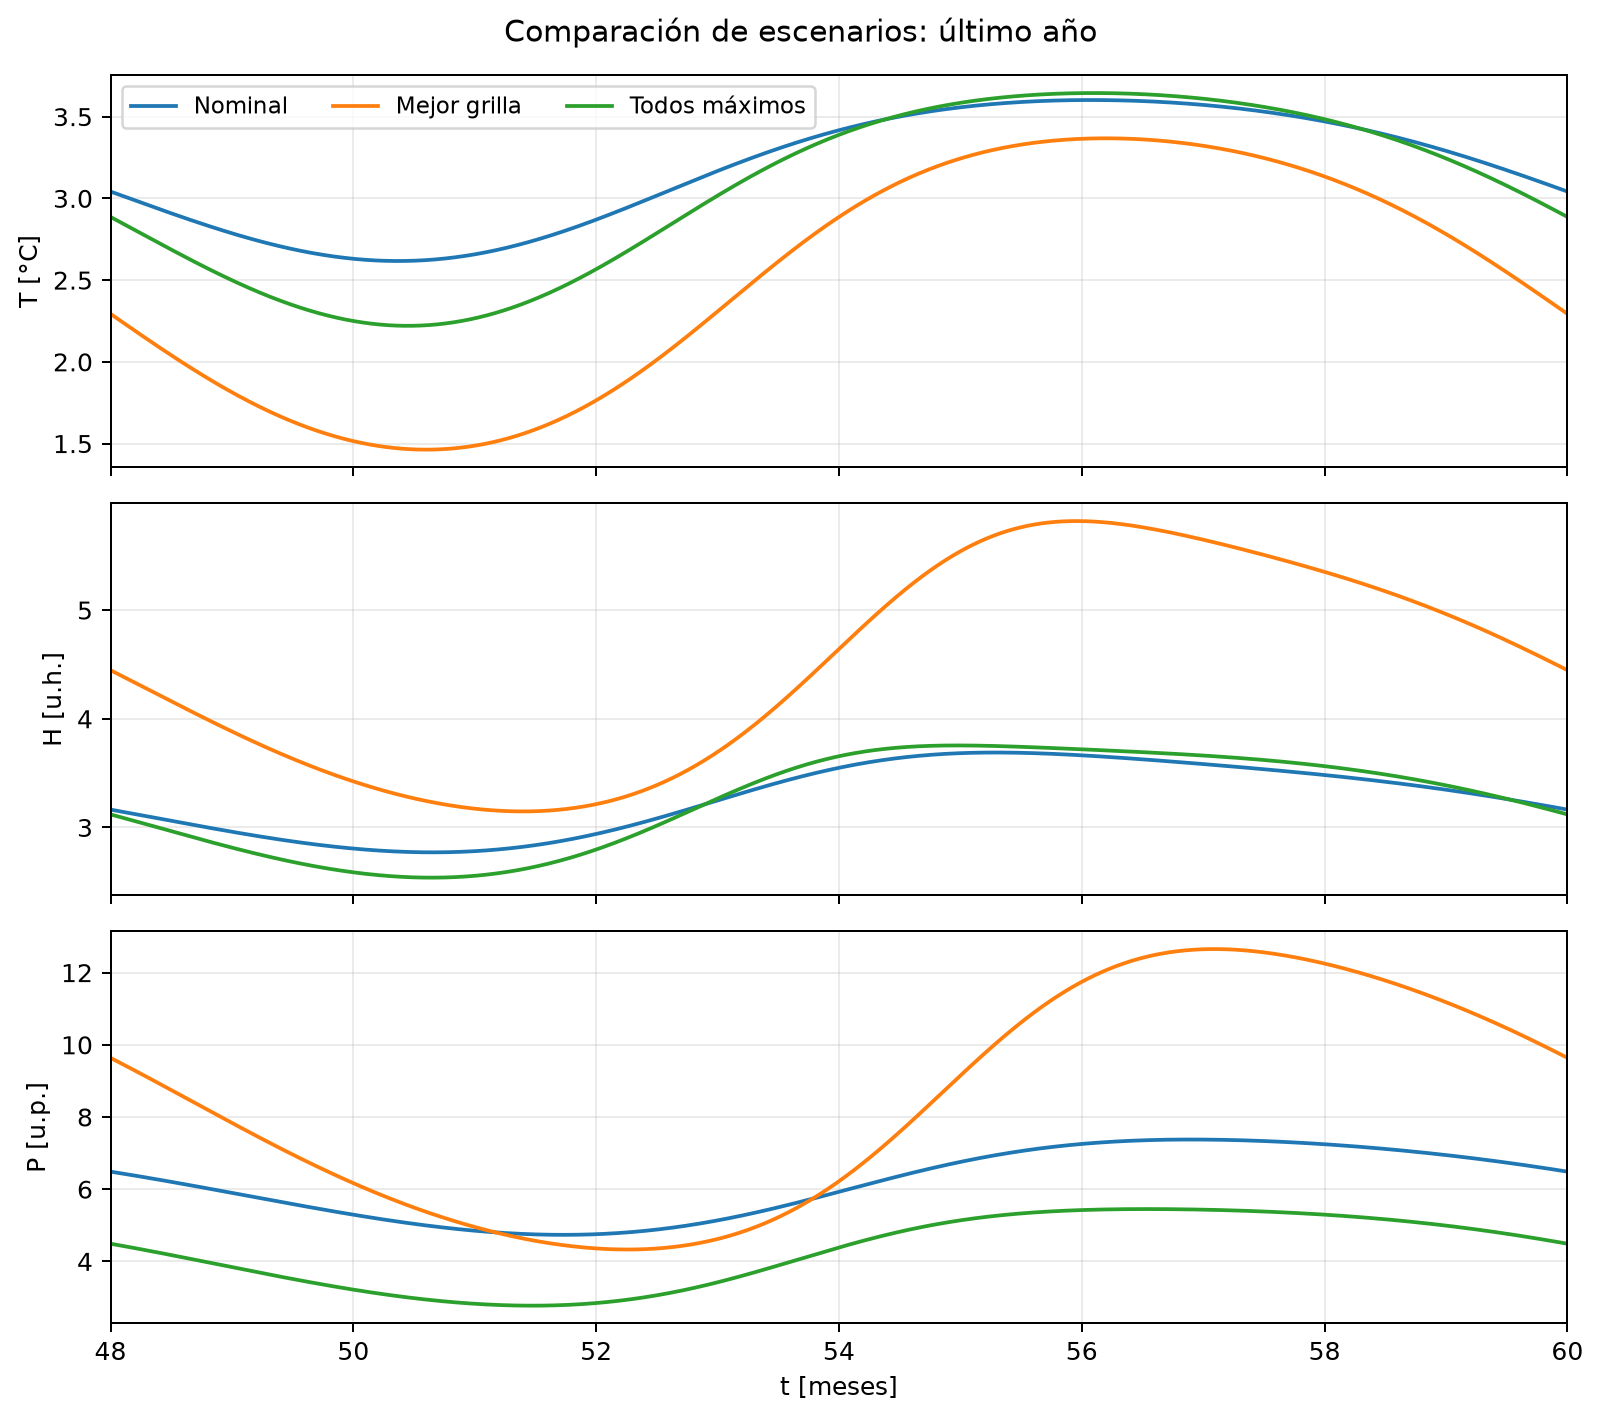
\includegraphics[width=\linewidth]{img/07_comparacion_ultimo_ciclo.png}
    \caption{Comparación entre el escenario nominal y el escenario de
    máxima severidad durante el último ciclo anual.}
    \label{fig:parte2-comparacion-ciclo}
\end{figure}

\begin{figure}[H]
    \centering
    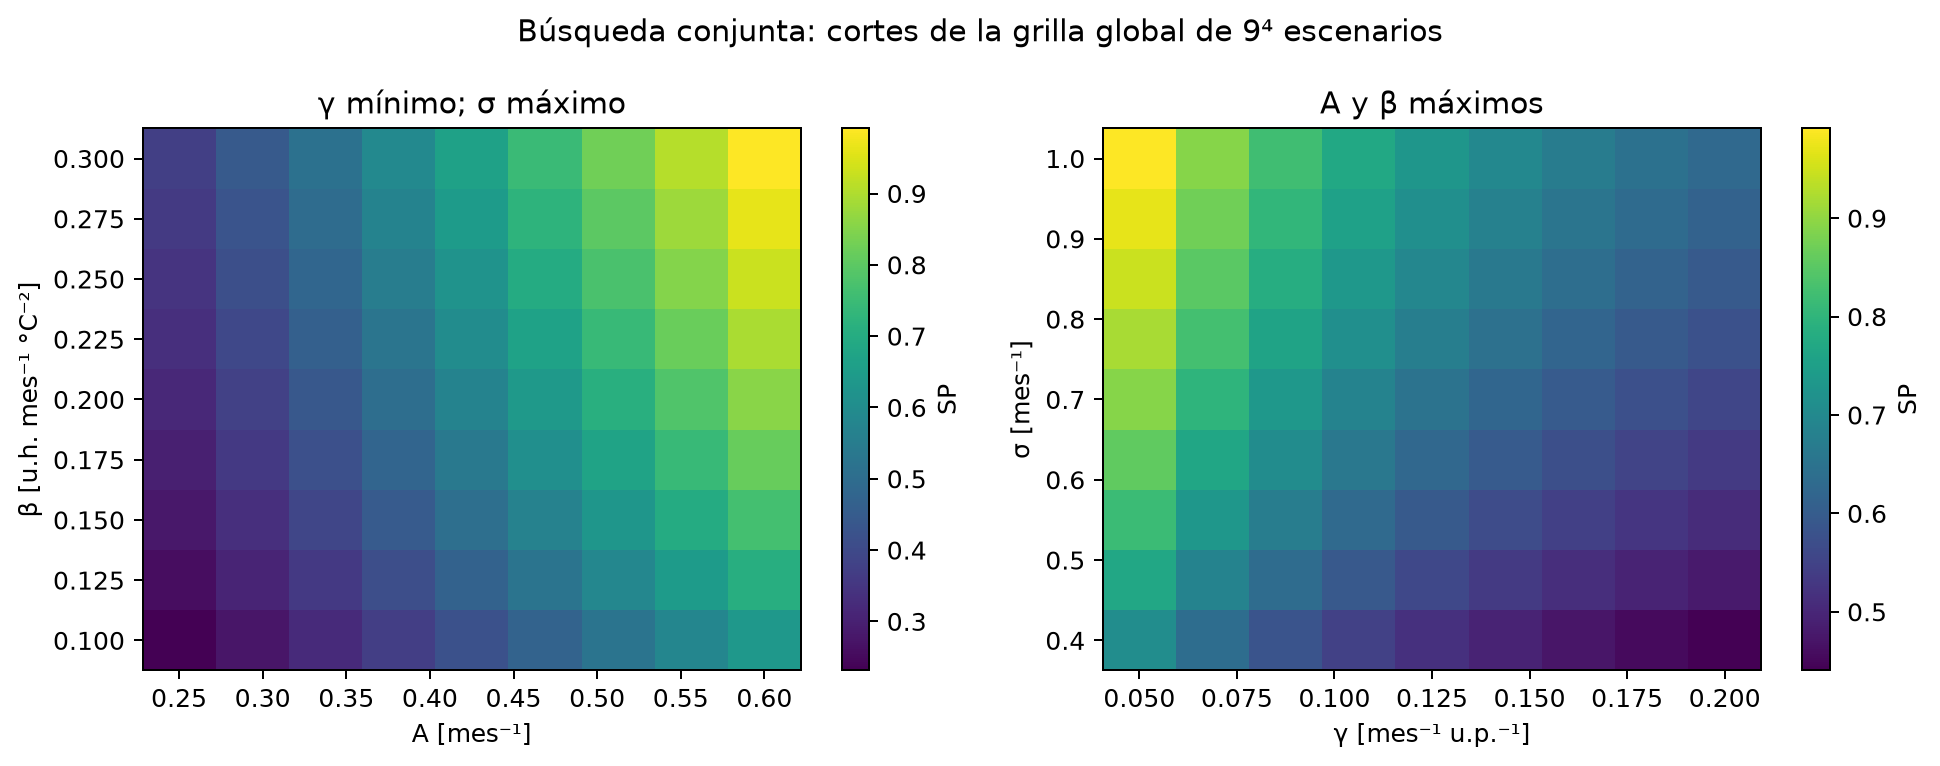
\includegraphics[width=\linewidth]{img/09_busqueda_conjunta.png}
    \caption{Resultados de la búsqueda conjunta. Los cortes mostrados
    mantienen fijos los otros dos parámetros según se indica en cada gráfico.}
    \label{fig:parte2-busqueda-conjunta}
\end{figure}

El mejor escenario tiene $S_P=0{,}9913$, unas $2{,}31$ veces el nominal, con
$P_{\max}$ y $P_{\mathrm{med}}$ mayores y un desfase similar
($0{,}894$ frente a $0{,}826$ meses). Sin embargo, \textbf{no} corresponde a
tomar todos los parámetros en su valor máximo: con $\gamma=0{,}20$ se obtiene
$S_P=0{,}626$, solo $1{,}46$ veces el nominal. El signo y la función de cada
término explican por qué:
\begin{itemize}
    \item $A$ multiplica $\cos(\omega t-\pi)$ en $R(t)$, que impulsa a $T$.
    Aumentarlo intensifica la oscilación de $T$, que se transmite a $H$ y $P$
    por las fuentes cuadráticas. Efecto positivo sobre $S_P$.
    \item $\beta$ multiplica $+\beta T^2$ en $dH/dt$: es una fuente de
    humedad. Efecto positivo.
    \item $\sigma$ multiplica $-\sigma P$ en $dP/dt$: es un sumidero de $P$.
    Al aumentarlo, $P$ sigue más rápido a $\delta H^2$ y el contraste entre
    máximo y mínimo crece. Efecto positivo.
    \item $\gamma$ multiplica $-\gamma HP$ en $dH/dt$: es un sumidero de
    humedad que crece con $P$. Aumentarlo reduce $H$, y con ella la fuente
    $\delta H^2$ de $P$. Efecto negativo.
\end{itemize}
Por lo tanto, $S_P$ crece al aumentar $A$, $\beta$ y $\sigma$ y al disminuir
$\gamma$, de modo que el máximo se alcanza con $\gamma$ en su mínimo. Además,
$S_P$ mide una amplitud relativa y no la cantidad de lluvia: con todos los
parámetros en su máximo, $P_{\max}=5{,}450$ u.p.\ es menor que el nominal
($7{,}376$ u.p.), aunque $S_P$ sea mayor.

El mejor escenario es el mejor entre los valores evaluados: las tres grillas
(inicial, global y local) dieron el mismo ganador, pero, como solo se
probaron valores discretos de los parámetros, esto no demuestra que sea el
máximo absoluto de $S_P$ dentro de los intervalos.